% paper_e.tex  
%    A manuscript sample for submission to Transactions of the Institute of 
%    Systems, Control and Information Engineers

%Authors: Please do not make any changes on the commands below.
%%%%%%%%%%%%%%%%%%%%%%%%%%%%%%%%%%%%%%%%%%%%%%%%%%%%%%%%%%%%%%%%%%%%%%%%%%%%%%
\documentclass[E]{scitrans}
%\usepackage{graphicx}
\usepackage{color}
\usepackage{math}
\usepackage{bm}
\usepackage{here}
%\usepackage[dvipdfmx]{graphicx,xcolor}
\usepackage[dvipdfmx]{epsfig}
%
\appearyear{0000}
\vol{0}
\numberinvol{0}
\setcounter{page}{1}
\setcounter{volumepage}{1}
\Transaction
%%\Shortpaper
\ForSubmission
%Authors: Please do not make any changes on the commands above.
%%%%%%%%%%%%%%%%%%%%%%%%%%%%%%%%%%%%%%%%%%%%%%%%%%%%%%%%%%%%%%%%%%%%%%%%%%%%%%


%%Authors: If you wish to use packages, please include them here.
%%         Note that only "amsfonts" and "psfrag" packages are available.
%%         The "latexsym" package has been already included.
%\usepackage{amsfonts}
%\usepackage{psfrag}

%Authors: Please follow the format below to fill in: paper's title, authors' 
%         names and affiliations, paper's condensed title and authors' names,
%         abstract and keywords.
%%%%%%%%%%%%%%%%%%%%%%%%%%%%%%%%%%%%%%%%%%%%%%%%%%%%%%%%%%%%%%%%%%%%%%%%%%%%%%
\begin{document}

\title{DESIGN OF A TWO-PIECE BRASSIERE CUP TO FIT BREAST DATA POINTS TOWARD ITS AUTOMATION}

\author{Kotaro {\sc Yoshida}${}^\dagger$, Hidefumi {\sc Wakamatsu}${}^\dagger$, Eiji {\sc Morinaga}${}^\ddagger$, and Takahiro {\sc Kubo}${}^\S$}

%Authors: Please write paper's short title and authors' names.
\headingtitle{DESIGN BRASSIERE CUP TO FIT BREAST DATA POINTS}
\headingauthors{{\sc Yoshida}, {\sc Wakamatsu}, {\sc Morinaga} and {\sc Kubo}}

%Authors: Please copy the abstract of your paper.
\abstract{
       A brassiere cup consists of several patterns. Traditionally, it is designed by repeatedly creating a paper cup model and verifying its three-dimensional (3D) shape. Reducing such trial and error will enhance the design efficiency. A method to partly automate the design of two-dimensional shapes in the patterns for a two-piece brassiere cup is proposed when the target 3D shape is given as a cloud of data points. It is assumed that the surface of the model is composed of several developable surfaces because the model is made of paper and not cloth. If two lines lying on a developable surface are given, the shape of the surface can be determined. Consequently, a two-piece brassiere cup can be designed by minimizing the error between the surface and the given data points. Here, we mathematically verify that our proposed method can reproduce the original developable surface.
}

%Authors: Please do not make any changes on the commands below.
%%%%%%%%%%%%%%%%%%%%%%%%%%%%%%%%%%%%%%%%%%%%%%%%%%%%%%%%%%%%%%%%%%%%%%%%%%%%%%
\maketitle
\acceptdate{August 1, 1995}
\address{*}{\AcceptDate}
%Authors: Please do not make any changes on the commands above.

%%% In accordance with the ISCIE policy on overlapping conference/journal submissions, if the material of this paper originates from conference papers published in the proceedings of conferences or symposia organized by the ISCIE as preliminary report, the following line should be written at the footnote in the first page of this paper.
\address{*}{The material of this paper was partially presented at the International Symposium on Flexible Automation 2020 which was held in July, 2020.}

%%%%%%%%%%%%%%%%%%%%%%%%%%%%%%%%%%%%%%%%%%%%%%%%%%%%%%%%%%%%%%%%%%%%%%%%%%%%%%

%Authors: Please write down authors' affiliations and addresses.
\address{**}{Graduate School of Engineering,
	Osaka University;
	Yamadaoka, Suita city, Osaka 565-0871, JAPAN}
\address{***}{Graduate School of Humanities and Sustainable System Sciences,Osaka Prefecture University, 1-1, Gakuencho, Naka-ku, Sakai, Osaka 599-8531, Japan}
\address{****}{Wacoal Holdings Corporation;
	Nakajima-cho, Kisshoin, Minami-ku,Kyoto 601-8530, JAPAN}

%Authors: Please write down the keywords of your paper.
\keywords{design, simulation, theory of surfaces, automation}

%Authors: Please remove \input and write down the body of your paper.
%\section{Introduction}
This document describes how to use the \LaTeX2e class file, named 
``{\tt scitrans.cls}'', for Transactions of the Institute of Systems, 
Control and Information Engineers (ISCIE). 

{\tt scitrans.cls} works together with the following nine files: 
\begin{itemize}
\item {\tt scitrans.cls}
\item {\tt sci209.sty, scij.sty, scie.sty, scims.sty}
\item {\tt JT1scimc.fd, JT1scigt.fd}
\item {\tt JY1scimc.fd, JY1scigt.fd}
\end{itemize}
Please make sure that all these files are placed in the same directory 
as the source file and should not be modified.


\section{Sections, etc.}
This is an example of \verb+\section{ }+.

\subsection{Subsections}
This is an example of \verb+\subsection{ }+.

\subsubsection{Sub-Subsections}
This is an example of \verb+\subsubsection{ }+.


\paragraph{Paragraphs}
This is an example of \verb+\paragraph{ }+.
Please insert a blank line before \verb+\paragraph{ }+.


\subparagraph{Subparagraphs}
This is an example of \verb+\subparagraph{ }+.
Please insert a blank line before \verb+\subparagraph{ }+.


\section{Theorems, etc.}
In the {\tt scitrans.cls} class file,
theorems and related structures such as definition, lemma, proposition,
corollary, example, assumption, remark and proof are handled. 
For example,

\begin{theorem}
\label{theorem:1}
This is an example of the theorem environment.
The usage of the lemma, definition, proposition, corollary,
example and assumption environments 
are the same as that of the theorem environment.
\end{theorem}

\begin{proof}
This is an example of the proof environment. 
At the end of each proof, asterisks ``**'' are automatically placed
as the Q.E.D.\ symbol,
whereas they will be replaced by the symbol ``$\Box$'' in the final manuscript.
\end{proof}

\begin{remark}
\label{remark:1}
This is an example of the remark environment. 
\end{remark}

If the author wishes to declare a new theorem-like environment, 
\verb+newtheoremenv+ and \verb+newparenenv+ can be used.
For example,

\begin{newtheoremenv}{Question}
This is an example of declaring a new environment by \verb+newtheoremenv+.
\end{newtheoremenv}
\begin{newparenenv}{Answer}
This is an example of declaring a new environment by \verb+newparenenv+.
\end{newparenenv}



\section{Equations}
Equations are created by the traditional {\tt equation} environment. 
In order to produce multiline equations,
the {\tt eqnarray} environment can be used.
For example, 

\begin{eqnarray}
        \dot{\mbf{x}}(t) & = & A \mbf{x}(t) + B \mbf{u}(t) 
                               + \sum_{k=1}^N \Gamma_k \mbf{d}k(t)
                \label{eq:1}\\
        \mbf{y}(t) & = & C \mbf{x}(t) + D \mbf{u}(t)
                \label{eq:2}\\
        \mbf{u}(t) & = & F \mbf{x}(t)
                \label{eq:3}
\end{eqnarray}

\begin{subequations}  \label{eq:4}  
  \begin{eqnarray}
    \lefteqn{ 
        \frac{1}{2\pi} \int_{-\infty}^\infty 
        {\rm Tr}\, \{ \mbf{G}\T(-j\omega) \mbf{G}(j\omega) \} \, d\omega 
     }    \hspace*{2\zw} \nonumber \\
    & = & 
    \frac{1}{2\pi} \int_{-\infty}^\infty 
    {\rm Tr}\, \{  B\T (-j\omega I -A\T)^{-1}C\T \nonumber \\
    &   & 
    \times C (j\omega I - A)^{-1}B \}\, d\omega 
               \label{eq:4a} \\
    & = & 
    \frac{1}{2\pi j}\int_{-j\infty}^{j\infty} 
    {\rm Tr}\, \left\{ 
    \left[ \begin{array}{c|c} 
       A & B \\ \hline 
       C & 0 \end{array} \right]^\sim  
    \left[ \begin{array}{c|c} 
       A & B \\ \hline 
       C & 0 \end{array} \right]
    \right\} \, ds  
              \label{eq:4b} 
\end{eqnarray}
\end{subequations}

In multiline equations,
please pay attention to the message ``\verb+Overfull \hbox+'', 
and the equations should be composed with the proper length.

With the \verb+subequations+ environment, sub-equation numbers such as 
\Req{eq:4a}, \Req{eq:4b} can be achieved.
In equations, bold fonts can be output by using \verb+\mbf+ command.
The superscript ${\rm T}$ which expresses the transpose of a matrix and $\hinf$ 
can be achieved by \verb+\T+ and \verb+\hinf+ respectively.

For in-line equations, please use $\displaystyle \sum_{k=1}^N$
instead of $\sum_{k=1}^N$.
Similarly, the rule is applicable to \verb+\lim+, \verb+\max+, \verb+\min+,
etc.
For super and subscripts,
please use $X_a^b$ (\verb+$X_a^b$+) instead of ${X_a}^b$ (\verb+${X_a}^b$+).


\section{Figures and Tables}
%----------------------------
\begin{figure}[b]
        \centering
	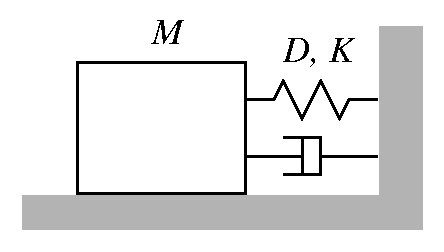
\includegraphics[width=5cm,clip]{tmp.eps}
        \caption{Mass-spring-damper system}
        \label{fig:1}
\end{figure}
%----------------------------
%
%----------------------------
\setlength{\unitlength}{10mm}
%

\begin{figure}[b]
        \centering
%
        \begin{picture}(4.5,1)(0,0)
                \thicklines
                \put(0,0.5){\vector(1,0){1.5}}
                \linethickness{1.2pt}
                \put(1.5,0){\framebox(1.5,1){$G(s)$}}
                \thicklines
                \put(3,0.5){\vector(1,0){1.5}}
        \end{picture}
%
        \caption{Plant}
        \label{fig:2}
\end{figure}
%----------------------------
%
%----------------------------
\begin{figure}[b]
        \centering
%
        \begin{picture}(5.5,2.5)(0,0)
                \thicklines
                \put(0,2){\vector(1,0){0.85}}
                \put(0.7,2.2){\makebox(0,0){$ \scriptstyle + $}}
                \put(1,2){\circle{0.3}}
                \thicklines
                \put(1.15,2){\vector(1,0){0.85}}
                \linethickness{1.2pt}
                \put(2,1.5){\framebox(1.5,1){$G(s)$}}
                \thicklines
                \put(3.5,2){\line(1,0){1}}
                \put(4.5,2){\circle*{0.08}}
                \put(4.5,2){\vector(1,0){1}}
                \put(4.5,2){\line(0,-1){1.5}}
                \put(4.5,0.5){\vector(-1,0){1}}
                \linethickness{1.2pt}
                \put(2,0){\framebox(1.5,1){$H(s)$}}
                \thicklines
                \put(2,0.5){\line(-1,0){1}}
                \put(1,0.5){\vector(0,1){1.35}}
                \put(0.8,1.7){\makebox(0,0){$ \scriptstyle - $}}
        \end{picture}
%
        \caption{Feedback control system}
        \label{fig:3}
\end{figure}

Graphics files (EPS files) can be inserted into a manuscript by 
\verb+\includegraphics+ command of the {\tt graphicx} package
(see \rfig{fig:1}). 
Here are some examples to insert graphics into a manuscript.
The {\tt picture} environment is also available
to draw figures (see \rfig{fig:2,fig:3}).

%
\begin{table}[h]
  \centering
  \caption{Example of table ({\tt slashbox.sty})}
  \label{table:1}
        \vspace{0.5\baselineskip}
  \begin{tabular}{!l!*{2}{c|}c!}\hlinethick
  \backslashbox{Room}{Date}
    &\makebox[3em]{5/31} &\makebox[3em]{6/1} &\makebox[3em]{6/2}\\ \hlinethick
    Room A	& --- & --- & --- \\ \hline
    Room C12	& --- & --- & --- \\ \hline
    Room F1201	& --- & --- & --- \\ \hlinethick
  \end{tabular}
\end{table}
%

Here is an example of a table. 
In the {\tt scitrans.cls},
the \verb+\tabular+ command has been extended for the ISCIE format.
The \verb+\tabular+ command provides the thin and thick lines.
The thin line can be achieved by the traditional way: ``\verb+|+''
for the vertical line and ``\verb+\hline+'' for the horizontal line.
The thick line can be achieved by ``\verb+!+'' and ``\verb+\hlinethick+''
for the vertical and horizontal thick lines respectively.

The {\tt arydshln.sty} is included in the {\tt scitrans.cls}
so that dashed lines are also available. 
Examples are shown in \rtab{table:2,table:3}.

%----------------------------
\begin{table}[hbt]
        \centering
        \caption{Commands for reference}
        \label{table:2}

        \vspace{0.5\baselineskip}

        \hdashlinewidth=8pt
        \hdashlinegap=4pt
        \begin{tabular}{!c|l!} \hlinethick
                Definition  & \verb+\rdefinition+ \\ \hdashline
                Theorem     & \verb+\rtheorem+ \\ \hdashline
                Lemma       & \verb+\rlemma+ \\ \hdashline
                Proposition & \verb+\rproposition+ \\ \hdashline
                Corollary   & \verb+\rcorollary+ \\ \hdashline
                Example     & \verb+\rexample+ \\ \hlinethick
        \end{tabular}
\end{table}
%----------------------------
%
%
%----------------------------
\begin{table}[hbt]
        \centering
        \caption{Commands for reference to equations, figures and tables}
        \label{table:3}

        \vspace{0.5\baselineskip}

        \hdashlinewidth=2pt
        \hdashlinegap=2pt
        \begin{tabular}{!l|l!} \hlinethick
                Equation                 & \verb+\req+ \\ \hdashline
                Equation in appendices   & \verb+\Req+ \\ \hdashline
                Equation with sub-number & \verb+\Req+ \\ \hdashline
                Figure                   & \verb+\rfig+ \\ \hdashline
                Table                    & \verb+\rtab+ \\ \hlinethick
        \end{tabular}
\end{table}
%----------------------------


\section{Citations}
Citations can be made with the \verb+\cite+ command\cite{foo1}. 
The \verb+\cite*+ command automatically places a word ``Ref.''
before the reference number as ``\cite*{foo1}''.

The multiple citation such as
\verb+\cite{foo1,foo2}+ and \verb+\cite{foo2,foo3,foo4}+ 
achieves \mbox{}\cite{foo1,foo2} and \mbox{}\cite{foo2,foo3,foo4} respectively.


\section{Cross-Referencing}
In order to reference the definition, theorem etc.,
please use the commands listed in \rtab{table:2},
for example: \verb+\rtheorem{theorem:1}+, \verb+\rremark{remarl:1}+.

\rtheorem{theorem:1} is an example of the \verb+\rtheorem+ command.

\rremark{remark:1} is an example of the \verb+\rremark+ command.

For referencing the equation,
figure and table, please use the commands listed in \rtab{table:3}.
These commands automatically add appropriate words before reference numbers.
For example, 
%the commands \verb+\req{eq:1}+, \verb+\rfig{fig:1}+ and \verb+\rtab{table:1}+
achieve 

\begin{itemize}
  \item \verb+\req{eq:1}+ $\quad\Longrightarrow\quad$ \req{eq:1}
  \item \verb+\rfig{fig:1}+ $\quad\Longrightarrow\quad$ \rfig{fig:1}
  \item \verb+\rtab{table:1}+ $\quad\Longrightarrow\quad$ \rtab{table:1}
\end{itemize}
The multiple referencing can be also achieved, for example,
\begin{itemize}
  \item \verb+\req{eq:1,eq:2,eq:3}+ $\quad\Longrightarrow\quad$
	\req{eq:1,eq:2,eq:3}
  \item \verb+\rfig{fig:1,fig:2}+ $\quad\Longrightarrow\quad$ \rfig{fig:1,fig:2}
  \item \verb+\rtab{table:1,table:2}+ $\quad\Longrightarrow\quad$
	\rtab{table:1,table:2}
\end{itemize}
In order to use the same format through the manuscript,
please do not use traditional 
\verb+\ref+ command.


\section{Others}
\subsection{Footnote}
The footnote is available with \verb+\footnote+ command%
\footnote{This is an example of the {\tt \textbackslash footnote} command.}.

\subsection{URL}
The {\tt scitrans.cls} provides the \verb+\url+ command to output a URL. 
For example, \url{http://www.iscie.or.jp/} can be achieved by 
\verb+\url{http://www.iscie.or.jp/}+. 
Also, {\tt \url{http://www.iscie.or.jp/}}  can be achieved by 
\verb+{\tt \url{http://www.iscie.or.jp/}}+. 


\acknowledgement
The \verb+\acknowledgement+ command can be used to state the acknowledgements. 


\begin{thebibliography}{9}
\bibitem{foo1}
        I.\ S.\ Cie: 
        The ISCIE style option; 
        {\it ISCIE Journal}, Vol.~0, No.~0, pp.~000--999 (1999)

\bibitem{foo2}
        R.\ E.\ Kalman: 
        A New Approach to Linear Filtering and Prediction Problems; 
        {\it Trans.\ of the ASME--J. of Basic Engineering}, Vol.~82 (Series D), 
        pp.~35--45 (1960)

\bibitem{foo3}
        A.\ Papoulis: 
        {\it Probability, Random Variables and Stochastic Processes}; 
        4th Edition, McGraw-Hill (2002)

\bibitem{foo4}
        Authors:
        Article title, {\it Book Title} (Editor(s), Ed(s).), Publisher,
        pp.~00--99 (1999)
\end{thebibliography}



%% Appendix
%
\appendix

This is an example of the \verb+\appendix+ command.
If there is only one section, please use \verb+\section*+ command. 
If there is more than one section, please use \verb+\section+ command.

\section{Equation in Appendix}
This is an example of \verb+\section+ command in the appendix. 
\begin{equation}
  u=Fx
\end{equation}

\section{Slash Line in Table}
In {\tt scitrans.cls}, {\tt slashbox.sty} is included so that slash 
lines are available in tables.
The followings are quoted from the manual of {\tt slashbox.sty} which is 
slightly modified for this document.

The usage is pretty straightforward, such as

\bigskip  %%Do not use this command in your manuscript.

\begin{tabular}{!l!*{3}{c!}}\hlinethick
\backslashbox{Room}{Date}
&\makebox[3em]{5/31}&\makebox[3em]{6/1}&\makebox[3em]{6/2}\\ \hlinethick
Room A&&&\\ \hline
Room C12&&&\\ \hline
Room F102&&&\\ \hlinethick 
\end{tabular}

\bigskip  %%Do not use this command in your manuscript.

\noindent
You may include a newline (\verb+\\+) in `Room' and/or `Date'.
Note that you will get spaces aside the slash line if there is a
wider column in the same column of a different line.
In such a case, you need to specify the width of the slashed column
by saying

\bigskip  %%Do not use this command in your manuscript.

\begin{tabular}{!l!*{2}{c!}} \hlinethick 
\backslashbox[40mm]{Room}{Date}
&\makebox[3em]{5/31}&\makebox[3em]{6/1}\\ \hlinethick 
Long Long Room Name&&\\ \hline
Room C12&&\\ \hline
Room F102&&\\ \hlinethick
\end{tabular}

\bigskip  %%Do not use this command in your manuscript.

The specified width is ignored if it is narrower than the natural
width of the column.

\verb+\(back)slashbox+ assumes by default that there is a blank space
of width \verb+\tabcolsep+ on both sides of the column.
Thus the slash line might exceed the boundary when you use \verb+@{}+ 
etc.

You can avoid it by specifying

\bigskip  %%Do not use this command in your manuscript.

\begin{tabular}{!@{\ $\bullet$\hspace*{3mm}}l!*{3}{c!}} \hlinethick 
\multicolumn{1}{!@{}l!}{\backslashbox[0pt][l]{Room}{Date}}
&\makebox[3em]{5/31}&\makebox[4em]{6/1}&\makebox[3em]{6/2}\\ \hlinethick
Room A&&&\\ \hline
Room C12&&&\\ \hline
Room F102&&&\\ \hlinethick 
\end{tabular}

\bigskip  %%Do not use this command in your manuscript.

\noindent
Here \verb+[l]+ tells the command that there is no extra space on the
left of this column.  You can use \verb+[r]+ and \verb+[lr]+ likewise.
You have to also specify the width of the column in this case, but it
can be 0pt.


\bigskip  %%Do not use this command in your manuscript.



\chosharyakureki

\authorbiography{Given-name, ,Family-name}{}{Member}{%
  Example of {\tt \textbackslash authorbiography}
  command. If you wish to include your photograph, please use this command.
  Please submit your photo after acceptance for publication.
  Please write down your biography here....
  Please write down your biography here....
  Please write down your biography here....
  Please write down your biography here....
  Please write down your biography here....
  Please write down your biography here....
  }

\authorbiography{Given-name, ,Family-name}{}{Non-Member}{%
  Example of {\tt \textbackslash authorbiography}
  command. If you wish to include your photograph, please use this command.
  Please submit your photo after acceptance for publication.
  Please write down your biography here....
  Please write down your biography here....
  Please write down your biography here....
  Please write down your biography here....
  Please write down your biography here....
  Please write down your biography here....
  }

\authorbiography*{Given-name, ,Family-name}{}{Member}{%
  Example of {\tt \textbackslash authorbiography$\ast$} command.
  If you do not wish to include your photograph, please use this command.
  Please write down your biography here....
  Please write down your biography here....
  Please write down your biography here....
  Please write down your biography here....
  }


\section*{INTRODUCTION}

Developable surfaces can be unfolded into a plane without expanding or contracting. They are widely used in many industries from shipbuilding to manufacturing of clothing because they can represent surfaces made of leather, paper, or sheet metal. It is important to design two-dimensional (2D) shapes that form the required three-dimensional (3D) shape by bending and joining. In this paper, we focus on production of brassieres, which is related to design of two-dimensional shapes of plates. 
Brassieres are manufactured to meet various demands, such as to Herein we focus on the production of brassieres, which is related to the design of 2D shapes of plates. Brassieres are manufactured to meet various demands such as enhancing a woman’s breast size, creating cleavage, or minimizing breast movement. Due to these diverse demands, the cup shape is a critical element when designing a brassiere. A brassiere cup is formed by several pieces of cloth called patterns and a wire. Figure 1 shows an example of a two-piece brassiere cup composed of an upper pattern, lower pattern, and lower line. 
\begin{figure}[h!]
	\centering
	\subfigure[upper pattern]{
		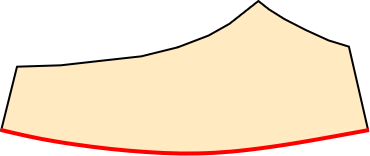
\includegraphics[width=0.45\columnwidth]{./figure/UpperPattern.png}
		\label{fig:pattern_U}
	}
	\hfil
	\subfigure[lower pattern]{
		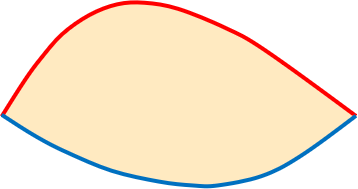
\includegraphics[width=0.45\columnwidth]{./figure/LowerPattern.png}
		\label{fig:pattern_L}
	}
	\\
	\subfigure[lower line]{
		
\includegraphics[width=0.35\columnwidth]{./figure/LowerWire.png}
		\label{fig:Wire}
	}
	\caption{Parts of a two-piece brassiere cup}
	\label{fig:patterns}
\end{figure}
 The three resulting curves are important to the design. The wire line corresponds to the boundary between the breast and body (\rfig{fig:TwoCurves}). The ridge line of the cup corresponds to the outline of a bust on a transverse plane, while the upper line connects the cup to the shoulder strap.  

%==============================================================%
In apparel industries, the form of a product is fixed by fashion designers and pattern makers. Fashion designers draw the product image, while pattern makers determine the pattern shapes to meet various demands of the ideal shape.
%%fig
\begin{figure}[h!]
	\centering
	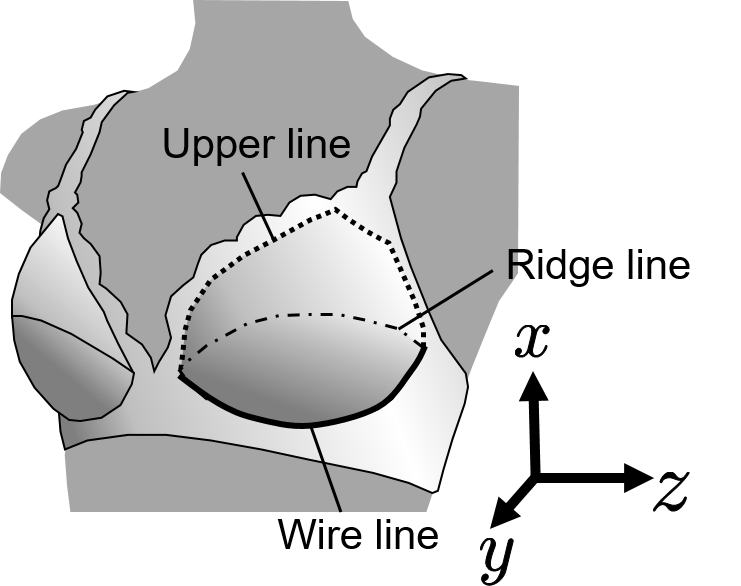
\includegraphics[scale=0.25]{./figure/Lines.png}
	\caption{Expression of a wire line, a ridge line and an upper line}
	\label{fig:TwoCurves}
\end{figure}
\rfig{fig:process} overviews the design process of a brassiere cup. Pattern makers first consider the functional requirement of a brassiere cup based on the breast shape, and then they determine the pattern shape. This design process is based on experience and intuition. Hence, pattern makers must verify the shapes with a paper model of the cup and repeatedly modify the shapes to realize the intended function. This process may cause unnecessary repetition. To improve the design efficiency of brassieres, trial and error should be minimized. Herein we strive to automate the steps indicated by the dotted line in \rfig{fig:process}. 
A previous study on the influence of design on the function of a brassiere cup found that fitting the breast has the largest impact\cite{c1}. Hence, this study proposes a method to design the pattern shapes of a brassiere cup to fit the given breast shape. Here, the given 3D breast shape is assumed to be a cloud of data points, which can be obtained easily by measurements.

\begin{figure}[h!]
	\centering
	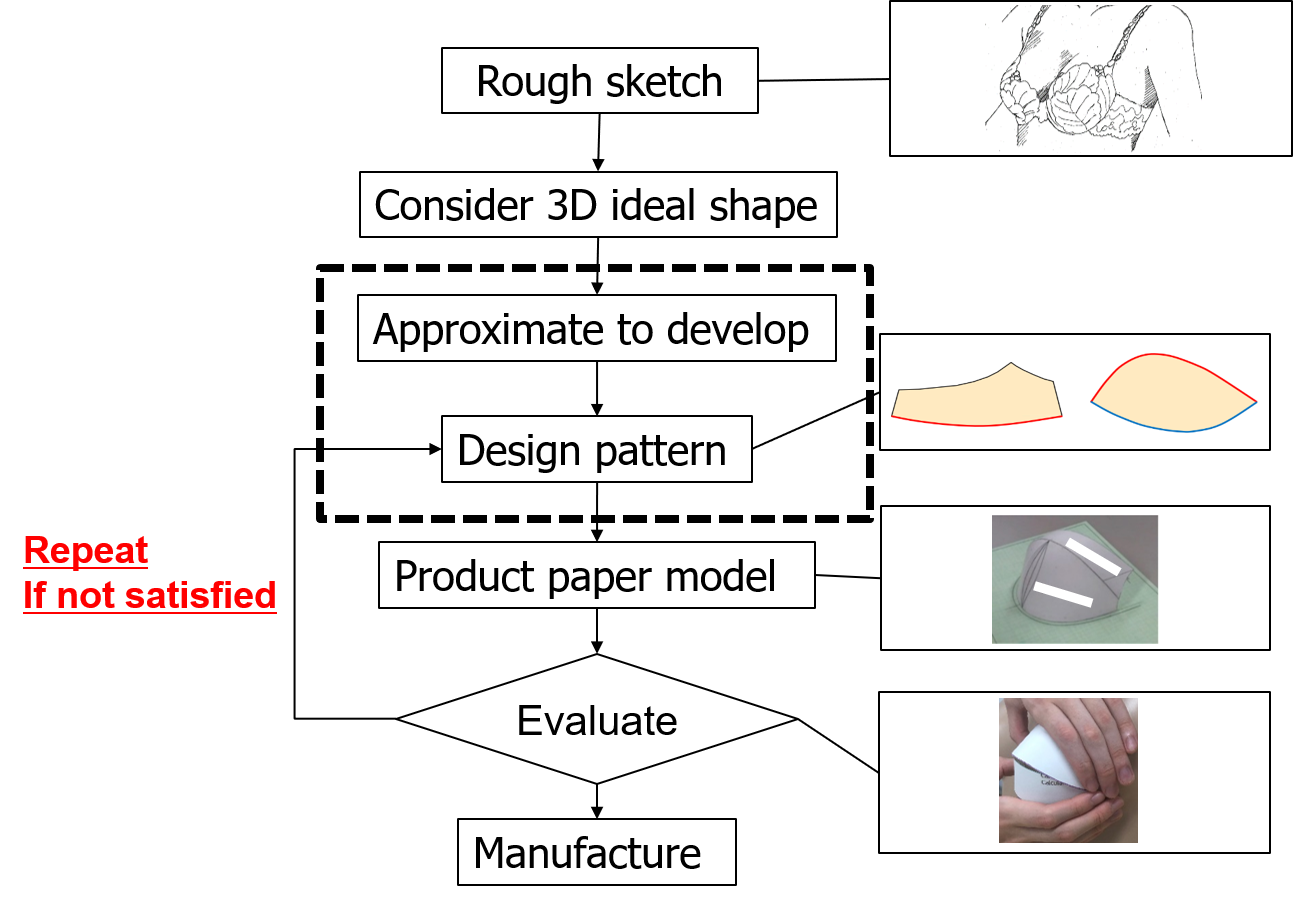
\includegraphics[width= 1.0 \columnwidth]{./figure/DesignProcess3.png}
	\caption{Design process of a brassiere cup}
	\label{fig:process}
\end{figure}

%==============================================================%
Because the cup shape is made by bending and sewing each pattern and is assumed to be inextensible, a cup model consists of several developable surfaces. With respect to modeling of developable surfaces, previously proposed modeling methods have focused on the geodesic line\cite{c2}, B-spline or NURBS surface\cite{c3,c4}, offsets of Bertrand curves, which coincide with each normal direction\cite{c5,c6}, and arbitrary curves\cite{c7}. Martin proposed a method to reconstruct a developable surface from its point clouds based on the Laguerre geometry\cite{c8}. Chen et al. proposed an algorithm to approximate a developable surface from its point cloud\cite{c9}. However, none of these methods reference the developed shape as they focus on a single developable surface. Manufacturing of a brassiere cup requires the pattern shapes (i.e., developed shapes of a cup) but not the 3D cup shape.

\chcolor{In a study to approximate developable surface, Yang et al. proposed a method to approximate surface with meshes composed of planar quadrilaterals\cite{cX1} and Odeo et al. proposed a method to define the developability of triangle meshes and appoximate them by a set of developable surfaces\cite{cX2}, and Martin et al. proposed a method to reconstruct surfaces by curved forming\cite{cX3}. But all of them only focus on approximating surface by developable surface, which means that they do not refer to the condition of a developable surface itself. In designing a brassire cup, it is required not only to fit a breast shape but also to satisfy some conditions. For example, the upper line has a point where it is connected with the shoulder strap. Hereafter, this point is called the connection point as shown in \rfig{fig:aboutCP}.} 
\begin{figure}[!h]
		\centering
		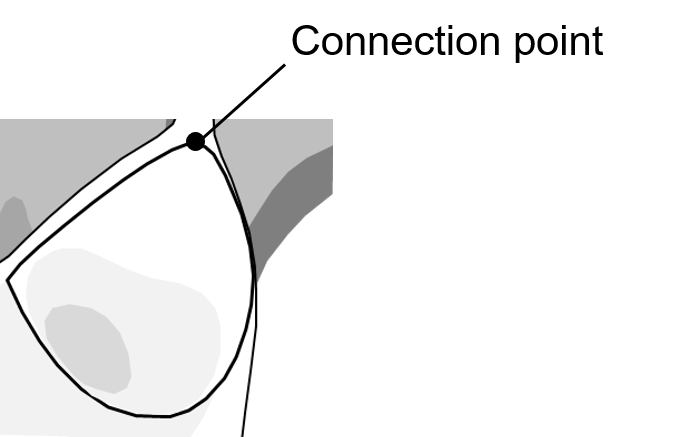
\includegraphics[width = 0.7\columnwidth]{./figure/Connection_Point.png}
		\caption{Expression about the connection point of a brassiere cup}
		\label{fig:aboutCP}
\end{figure}

In a study on brassieres, Wakamatsu et al. proposed a method to predict the 3D shape of a paper cup model when the 2D shape of a pattern is given\cite{c10,c11}. Hence, patterns can be evaluated without actually creating a paper model. However, repetitive modification of the pattern is still required to obtain the target 3D shape of the cup. Ito et al. developed a paper model CAD system based on the theory of developable surfaces\cite{c12}. If a 3D curve, which means a sewn curve, and a 2D curve, which means a piece to be sewn, are given, this system can identify the feasible region where the sewn surface does not intersect itself. Unfortunately, it is difficult to design the pattern shapes. That is, determining the shape of 2D curves is challenging with this system. 
We previously proposed a method to design the pattern shape and its developable surface from two lines: a wire line and a ridge line. These lines are obtained by solving the optimization problem when the design parameters are the geodesic curvatures of a pattern shape and the objective function is the error between generatrices determined by the geodesic curvature of a lower edge and the wire line and generatrices determined by the geodesic curvature of an upper edge and the ridge line. However, the previously proposed method requires an iterative process to solve the optimization problem for the intended shape\cite{MyRef,MyRef2}, which is time-consuming.
Brassiere patterns are typically comprised of two or three pieces. Herein we focus on a two-piece brassiere cup, and we propose a design method to improve the design efficiency when a cloud of its data points is given. 

%==============================================================%
%%%%%%%%%%%%%%%%%%%%%%%%%%%%%%%%%%%%%%%%%%%%%%%%%%%%%%%%%%%%%%%%%%%%%%
\section*{MODELING OF DEVELOPABLE SURFACE AND PATTERN SHAPE}

This section explains the numerical expressions of a developable surface. The curvature of a space curve on a surface can be divided into two: the normal curvature and geodesic curvature. The former is realized by deforming the surface, while the latter is realized by deforming a space curve. Deforming the surface does not change the geodesic curvature as long as the surface is not stretched. In the case of a brassiere cup, only the normal curvature can be manipulated by deforming the surface. Because the geodesic curvature cannot be manipulated by deforming the surface, it must be designed such that the space curve coincides with a boundary of the developable surface. 
Here, we propose a method to determine a developable surface using two curves that lie on the surface and design a pattern shape. Consider the case where the \textit{lower edge} is the curve connecting the lower wire (\rfig{fig:pattern_L}) and the \textit{upper edge} is that combining the upper cup (\rfig{fig:pattern_U}). Our method expresses the developable surface using the parameters of a space curve, the condition of two lines that lie on the developable surface, and their obtained pattern shape. \rfig{fig:obj_coord} depicts the object coordinate system on the lower edge of the cup surface, where the $\zeta$-axis always coincides with the tangential direction of the edge line and the  $ \eta $-axis always coincides with the surface normal direction. Deformation of the cup changes the posture of the object coordinate system. Thus, the infinitesimal displacement vector of each axial direction can be described by the infinitesimal rotational ratio vector $ \mbold{\omega} = \left[\omega_{\xi}\;\;\omega_{\eta}\;\;\omega_{\zeta}\right]^{\mathrm{T}}$ as

\begin{equation}\label{eq:ObjSys}
\left[\begin{array}{ccc} \xivec' & \etavec' & \zetavec' \end{array}\right] = \left[\begin{array}{ccc} \xivec & \etavec & \zetavec \end{array} \right] \mbold{\Omega}(\mbold{\omega}), 
\end{equation}
where a prime means a derivative of $s$, and $\mbold{\Omega}(\mbold{\omega})$ is represented as
\begin{equation}
\mbold{\Omega}(\mbold{\omega}) = \left[\begin{array}{ccc}
0 &-\omega_{\zeta} & \omega_{\eta} \\
\omega_{\zeta} & 0 &-\omega_{\xi} \\
-\omega_{\eta} & \omega_{\xi} &0
\end{array}\right]. 
\end{equation}

Then, the tangent vector is expressed as 
\begin{equation}
\zetavec(s) = \zetavec_0 + \int_{0}^{s} \left( \omega_{\eta} \xivec - \omega_{\xi} \etavec \right) ds,
\label{eq:zetav_eq}
\end{equation}
where $\zetavec_0$ represents the tangent vector at $s=0$. By integrating \req{eq:zetav_eq}, the position of the curve can be calculated as
\begin{equation}
\mbold{x}(s) = \mbold{x}_0 + \int_0^s \zetavec ds, 
\end{equation}
where $\mbold{x}_0$ indicates the position at $s=0$. 

\begin{figure}[thpb]
	\centering
	
\includegraphics[width = 0.8\columnwidth]{./figure/Object_Coordinates.png}
	\caption{Object coordinate system on the surface}
	\label{fig:obj_coord}
\end{figure}

First, consider the numerical expression of a developable surface constrained by a Gaussian curvature. In general, the normal curvature of a direction vector $\mbold{d}_{\theta} = \zetavec \cos \theta + \xivec \sin \theta $ can be described using coefficients of the first and the second fundamental forms $E, F, G, L, M$ and $N$ as
\begin{equation}\label{eq:def_kappa_theta}
\kappa_{\theta} = \frac{L \cos^2 \theta + 2M \sin \theta \cos \theta + N \sin^2 \theta}{E \cos^2 \theta + 2F \sin \theta \cos \theta + G \sin^2 \theta}.
\end{equation}
Then the Gaussian curvature $K$ and the mean curvature $H$, which characterize a surface, can be defined as extreme values of \req{eq:def_kappa_theta}: $ \kappa_{\max} $ and $ \kappa_{\min} $ as follows\cite{cX4}

\begin{eqnarray}
K &=& \kappa_{\max}  \kappa_{\min}  = \disfrac{LN-M^2}{EG-F^2}, \nonumber \\ 
H &=& \disfrac{\kappa_{\max} + \kappa_{\min}}{2} = \frac{EN-2FM+GL}{2(EG-F^2)}. 
\end{eqnarray}

Based on the theory of surface, the coefficients of the first fundamental form are represented as
\begin{equation}
E = \zetavec \cdot \zetavec = 1, F = \zetavec \cdot \xivec = 0, G = \xivec \cdot \xivec = 1.
\end{equation}
In addition, the coefficients of the second fundamental form are represented as
\begin{equation}
L = \zetavec' \cdot \etavec = -\omega_{\xi}, M = \xivec' \cdot \etavec = -\omega_{\zeta}.
\end{equation}
Then Gaussian curvature $K$ and the mean curvature $H$ are described by the following equations

\begin{eqnarray}
\label{eq:GC_expressed_omega}
K &=& -\omega_{\xi} N - \omega_{\zeta}^2, \\
H &=& \disfrac{-\omega_{\xi}+N}{2}.
\end{eqnarray}
A developable surface is defined as a surface with a Gaussian curvature $K = 0$. That is $\kappa_{\min}=0$. TThus, the mean curvature can be calculated as $2H=\kappa_{\max}$. The line direction coinciding with the direction $\mbold{d}_{\min}$ remains straight after a deformation. This straight line is referred to as a generatrix. In this paper, the principal directions are described using the angle $ \alpha $ as 
\begin{eqnarray}\label{eq:d1d2_eq}
\mbold{d}_{\max} &=& \zetavec \cos \alpha + \xivec \sin \alpha, \nonumber \\ 
\mbold{d}_{\min} &=& -\zetavec \sin \alpha + \xivec \cos \alpha.
\end{eqnarray}
The angle $ \alpha $ is referred to as the \textit{rib angle} in this paper.
By solving $ \kappa_{\theta} = 0 $, the rib angle $ \alpha $ can be calculated as
\begin{equation}\label{eq:alpha_eq}
\tan \alpha = -\frac{\omega_{\zeta}}{\omega_{\xi}}.
\end{equation}
From \req{eq:GC_expressed_omega}, $\kappa_1$ is calculated as 
\begin{equation}\label{eq:kappa1_eq}
\kappa_1 = -\frac{\omega_{\xi}^2 + \omega_{\zeta}^2}{\omega_{\xi}}.
\end{equation}
From above, a developable surface can be determined by $\mbold{\omega}$.

Next, consider the constraint of a developable surface when two curves lie on the surface. Let $s_a$ and $s_b$ be the arc length and $\mbold{x}_a(s_a)$, $\mbold{x}_b(s_b)$ be positions of each curve. We assume that these curves have ${\rm C}^2$ community at least. In general, developable surfaces are a special kind of ruled surface. When a surface is a ruled surface, the generatrix $ \mbold{g} $ is described as

\begin{equation}
\mbold{g} = \mbold{x}_b(s_b)-\mbold{x}_a(s_a).
\end{equation}

Note that $s_a$ can take an arbitrary value against $ s_b $. From \cite{MyRef2}, $ \zetavec_a$ and $\zetavec_b $, which are tangent vectors of $ \mbold{x}_a $ and $ \mbold{x}_b $, and $ \mbold{g} $ satisfy the following equation:
\begin{equation}
	\det (\zetavec_a, \zetavec_b, \mbold{g})=0. 
	\label{eq:Cond1}
\end{equation}
\req{eq:Cond1} indicates that the arc length of each curve is subordination, When two curves are corresponded to edge lines and $ s_b $ can be expressed as $s_b(s_a)$, $ \mbold{d}_{\min}  = \frac{\mbold{g}}{|\mbold{g}|}$ established. Then, a rib angle is calculated by \req{eq:d1d2_eq} as follows:
\begin{equation}\label{eq:alphaEq}
	\alpha_a = \sin^{-1} \mbold{d}_{\min} \cdot \zeta_a
\end{equation}
Then, using $ \mbold{d}_{\min} $ and $\alpha $, $ \mbold{\omega} $ can be represented as
\begin{equation}\label{eq:omegaVec}
\mbold{\omega} = \left[\begin{array}{c} -\det(\zetavec_a',\zetavec_a, \mbold{d}_{\min} ) \\ \zetavec_a' \cdot \mbold{d}_{\min} \\ \det(\zetavec_a',\zetavec_a, \mbold{d}_{\min} ) \tan \alpha_a \end{array}\right] 
\end{equation}
Therefore, when two curves that lie on the surface are given, a developable surface can be determined.

Now let’s consider how to determine the pattern shape from a developable surface. The planar curve generated by developing the space curve $ \mbold{x}_a $ is defined as the lower curve, whereas that generated by developing the space $ \mbold{x}_b $ is defined as the upper curve. \rfig{fig:PatternImage} shows the developed planar coordinate system $ vw $ so that $ v $-axis always coincides the line AB. Let $ \mu_a $ be the angle between the tangential direction of the lower edge and the $ v $-axis. 
If the curvature of the lower curve $ \omega_{\eta_a} $ is given, $ \mu_a $ is obtained as
\begin{equation}\label{eq:mu_eq}
\mu_a = \mu_0 + \int_{0}^{s_a} \omega_{\eta_a} ds_a,
\end{equation}
where $ \mu_0 $ represents the angle of the lower edge at $ s=0 $, which is discussed later. From \req{eq:mu_eq}, the planar position $ \mbold{x}_{ae} $ is described as
\begin{equation}\label{eq:x_LE}
\mbold{x}_{ae}  = \int_{0}^{s_a} \left[\begin{array}{cc} \cos \mu_a \\ \sin \mu_a \end{array}\right] ds_a
\end{equation}
With respect to \req{eq:mu_eq}, let $ a,b $ be defined as follows:
\begin{eqnarray}
a &=& \int_{0}^{L_a} \cos \left( \int_{0}^{s_a} \omega_{\eta_a} ds\right) ds_a, \\
b &=& \int_{0}^{L_a} \sin \left( \int_{0}^{s_a} \omega_{\eta_a} ds\right) ds_a. 
\end{eqnarray}
Then, $ \mu_0 $ can be calculated as follows:
\begin{equation}\label{eq:mu_0eq}
\mu_0 = \tan^{-1}\frac{b}{a}
\end{equation}
Let $ \mbold{x}_{be} $ be the planar position of an upper edge. Since the rib angle of a pattern $ \alpha_a $ and the length of a generatrix of a pattern $ |\mbold{g}| $ do not change by being developed, $ \mbold{x}_{be} $ can be calculated as 
\begin{equation}\label{eq:x_UE}
\mbold{x}_{be} = \mbold{x}_{ae} + |\mbold{g}| \left[\begin{array}{cc} \cos \left(\mu_a + \pi/2 + \alpha_a \right) \\ \sin \left(\mu_a + \pi/2 + \alpha_a \right)  \end{array}\right] 
\end{equation}
From above, a developed shape can be obtained when two curves, which lie on the developable surface, are given.
\begin{figure}[thpb]
	\centering
	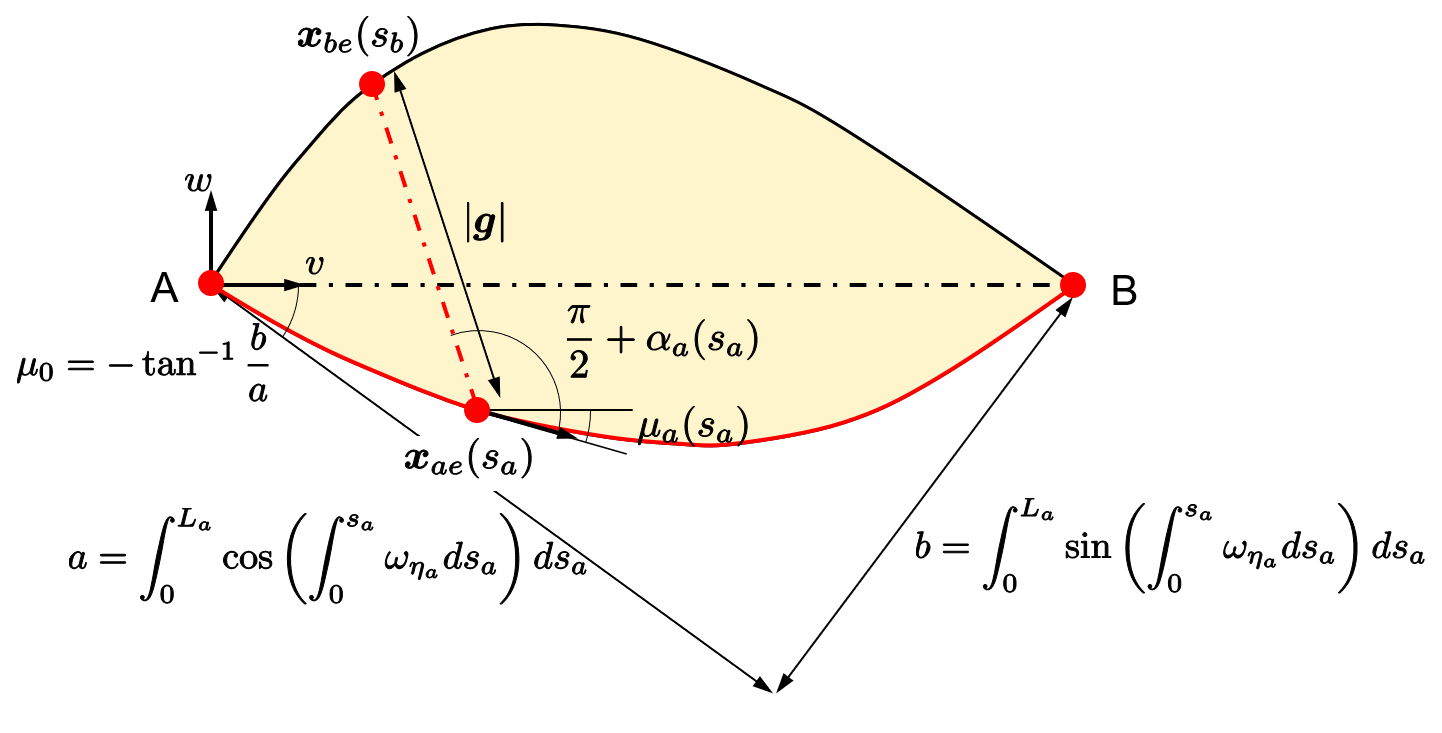
\includegraphics[width = \columnwidth]{./figure/PatternImage2.eps}
	\caption{Description of pattern shape using geodesic curvature of the lower curve}
	\label{fig:PatternImage}
\end{figure}
\section*{EXPRESSION OF THE DESIGN PROCESS AS AN OPTIMIZATION PROBLEM}
From section 2, the cup shape can be determined by three curves: a wire line, a ridge line, and an upper line. If the wire line is given, designing the parameters for the ridge and upper lines such that the degree of fitting to the 3D breast shape is minimized will enhance the design efficiency. This section formulates the optimization problem that our proposed method aims to solve.
%%%%%%%%%%%%%%%%%%%%%%%%%%%%%%%%%%%%%%%%%%%%%%%%%%%%%%%%%%%%%%%%%%%%%%
\subsection*{Formulation of the error between a point and a surface}
To formulate the degree of fitting to a 3D ideal shape, we formulate the error between a point and a surface. In general, the position $\mbold{X}(s,t)$ of a developable surface $S$ is expressed as
\begin{equation}\label{eq:Sur_eq}
\mbold{X}(s,t) = \mbold{x}(s) + t\mbold{d}_{\min}(s)
\end{equation}
The distance $\varepsilon(\mbold{p})$ between a point $\mbold{p}$ and a developable surface is formulated by the difference vector $\mbold{\delta}=\mbold{p}-\mbold{X}(s,t)$ as
\begin{equation}\label{eq:eps_eq}
\varepsilon(\mbold{p})=\min_{s,t}{|\mbold{\delta}|}
\end{equation}
When a set of surface parameters $ (s^*,t^*) $ satisfies to minimize \req{eq:eps_eq}, $\mbold{\delta}$ is parallel to $ \etavec $. Therefore, the following equations are satisfied
\begin{equation}\label{eq:d_mindoteq}
\mbold{d}_{\min} \cdot (\mbold{p} - \mbold{X}(s^*,t^*)) = 0
\end{equation}
\begin{equation}\label{eq:d_maxdoteq}
\mbold{d}_{\max} \cdot (\mbold{p} - \mbold{X}(s^*,t^*)) = 0
\end{equation}
By solving \req{eq:d_mindoteq}, $ t^* $ is described as
\begin{equation}\label{eq:t*_eq}
t^* = \mbold{d}_{\min} \cdot (\mbold{p}-\mbold{X}(s^*))
\end{equation}
By using \req{eq:t*_eq} and solving \req{eq:d_maxdoteq}, $ s^* $ can be determined.

Let $ s_w,s_r,s_u $ be the arc lengths of the lower wire, ridge line, and upper line and let $ \mbold{\omega}_W (s_w ),\mbold{\omega}_R (s_r ),\mbold{\omega}_U (s_u ) $ be vectors to characterize each of them, respectively. From \req{eq:Cond1}, $ s_r,s_u $ can be expressed as functions of $ s_w $: $ s_r (s_w ),s_u (s_w ) $. As mentioned, a two-piece brassiere cup is composed of two developable surfaces $ S_L $ and $ S_U $. Let $ D $ be a set of coordinates of points on a breast, $ D_L = \{\mbold{p}_{L,i} \in D \} $ be a set of points to evaluate the surface $ S_L $, and $ D_U = \{\mbold{p}_{U,i} \in D \} $ be a set of points to evaluated the surface $ S_U $. Note that $ D_U = D \backslash D_L $. Whether a point $ \mbold{p}_k $ is classified to the set of $ D_U $ or the set of $ D_L $ can determined with the length of the nearest generatrix.

First, using \req{eq:d_mindoteq,eq:d_maxdoteq,eq:t*_eq}, the nearest surface parameters $ (s_w^*, t_w^*) $ of the lower cup to the point $ \mbold{p}_k $ can be derived. Then, the nearest point $ \mbold{X}(s^*, t^*) $ on the lower cup surface to the point $ \mbold{p}_k $ can be derived. Let $ t_{\max}=|\mbold{x}_R (s_r (s_w^* ))-\mbold{x}_W (s_w^* )| $ be the length of a generatrix on the wire line. If $ t_{\max} > t_w^*(s_w^*) $, that is, if the perpendicular projection point of the point $ \mbold{p}_k $ to the surface $ S_L $ is included in the lower cup, the point $ \mbold{p}_k $ is classified to the set $ D_L $. Otherwise, it is classified to the set $ D_U $. 
\begin{figure}[thpb]
	\centering
	\subfigure[$ t^*\leq t_{\max} $]{
		
\includegraphics[width=0.45\columnwidth]{./figure/NotExceeding.png}
		\label{fig:inD_L}
	}
	\hfil
	\subfigure[$ t^* > t_{\max} $]{
		
\includegraphics[width=0.45\columnwidth]{./figure/Exceeding.png}
		\label{fig:inD_U}
	}
	\caption{Relationship between $ t^*$ and $t_{\max}$.}
	\label{fig:which_in}
\end{figure}

Thus, we can classify point data on a breast into two sets once two developable surfaces for the lower and the upper cup are determined.

From above, the error between the surface of a two-piece brassiere cup and its data points can be formulated:
\begin{equation}\label{eq:Lambda_eq}
\Lambda(D) = \sum_{i=1}^{N_L} \varepsilon(\mbold{p}_{L,i}) + \sum_{i=1}^{N_U} \varepsilon(\mbold{p}_{U,i}).
\end{equation}
By finding two developable surfaces that minimize the error described by \req{eq:Lambda_eq}, the appropriate pattern shapes can be determined.


\subsection*{Formulation of Objective Function and Conditions}
To consider the optimization conditions, we first explain the conditions for the parameters of the ridge line and the upper line. $ \omega_{\zeta} $ does not affect the shape of the space curve. Therefore, the following conditions are added 
\begin{eqnarray}\label{eq:conds_omgZt}
\omega_{\zeta_R}(s_r(s_w)) &=& 0 \;\; \forall s_w\in[0,L_L], \\
\omega_{\zeta_U}(s_u(s_w)) &=& 0 \;\; \forall s_w\in[0,L_L]. 
\end{eqnarray}
Then the following conditions must be satisfied to design the arc length
\begin{equation}\label{eq:conds_arc1}
	s_r(s_w) \geq 0 \;\; \forall s_w\in[0,L_L], 
\end{equation}
\begin{equation}\label{eq:conds_arc2}
	s_u(s_w) \geq 0 \;\; \forall s_w\in[0,L_L], 
\end{equation}
\begin{equation}\label{eq:conds_arc3}
	s_r'(s_w) \geq 0 \;\; \forall s_w\in[0,L_L], 
\end{equation}
\begin{equation}\label{eq:conds_arc4}
	s_u'(s_w) \geq 0 \;\; \forall s_w\in[0,L_L].
\end{equation}
In general, the end positions of the ridge and upper lines are aligned to the end point of the wire line. Therefore, the following equations must be satisfied 
\begin{equation}\label{eq:conds_endp1}
	\mbold{x}_R (s_r(s_w)) = \mbold{x}_L(s_w), 
\end{equation}
\begin{equation}\label{eq:conds_endp2}
	\mbold{x}_U (s_u(s_w)) = \mbold{x}_L(s_w).
\end{equation}

To guarantee that $ S_L $ and $ S_U $  are developable surfaces, the following equations must be satisfied 
\begin{equation}\label{eq:conds_DevSur1}
	\int_{0}^{L_L} \det (\zetavec_R(s_r(s_w)), \zetavec_W(s_w), \mbold{g}) ds_w = 0,
\end{equation}
\begin{equation}\label{eq:conds_DevSur2}
	\int_{0}^{L_L} \det (\zetavec_U(s_u(s_w)), \zetavec_W(s_w), \mbold{g}) ds_w = 0.
\end{equation}
Next, consider a “fuzzy” condition for a brassiere cup. As mentioned, the upper line has a connection point as shown in \rfig{fig:aboutCP}. But it is typically given as a fuzzy condition in the design process. This can lead to an unexpected error in the optimization problem. Therefore, we propose the following equation to deal with this fuzzy condition $ y \simeq Y $:
\begin{equation}\label{eq:FuzzyEq}
C(y,Y) = k_1 \exp( k_2(y-Y)^2 )
\end{equation}
where $ k_1 $ and $ k_2 $ are the variables to adjust the range that satisfies this condition. By adding this equation to the objective function, the fuzzy condition can be handled. Here, we assume that the position $ \mbold{X}_C $ to connect the upper line and the shoulder strap is given. Then the objective function $ V $ is described as
\begin{equation}\label{eq:ObjectFunc}
V = \Lambda(\mbold{D}) + \sum_{i=0}^{2} C(\mbold{x}_U \cdot \mbold{e}_i , \mbold{X}_C \cdot \mbold{e}_i)
\end{equation}
where $\mbold{e}_0 $ ,$\mbold{e}_1 $ and $\mbold{e}_2 $ are represented as unit vectors of $ x $,$ y $ and $ z $-axis. Solving this optimization under these constraints can provide the shape of the brassiere cup to fit the data points of a breast.

\subsection*{Procedure to Solve the Optimization Problem}
Prior to explaining the procedure to solve the optimization problem, we explain how to eliminate the condition. To satisfy  \req{eq:conds_arc1,eq:conds_arc2,eq:conds_arc3,eq:conds_arc4}, $ s_r (s_w),s_u (s_w) $ are described using arbitrary functions $ \upsilon_r(s_w),\upsilon_u(s_w) $ as
\begin{eqnarray}
s_r(s_w) &=& s_{r_0} + \int_{0}^{s_w} \upsilon_r^2 ds_w, \\
s_u(s_w) &=& s_{u_0} + \int_{0}^{s_w} \upsilon_u^2 ds_w. 
\end{eqnarray}
The initial position is assumed to be the wire line. Then the ridge and upper lines are aligned such that $ s_{r_0}=s_{u_0}=0 $. Let a composite function of $ s_r(s_w) $ and arbitrary function $ g(s_r) $ be defined as $ \tilde{g}(s_w) $, and a composite function of $ s_u (s_w ) $ and arbitrary function $ g(s_w) $ be defined as $ \hat{g}(s_w) $. From \req{eq:ObjSys}, the object coordinate system of the ridge and upper lines can be expressed as 
\begin{equation}\label{eq:tildeobj}
\left[\begin{array}{ccc} \tilde{\xivec}_R' & \tilde{\etavec}_R' & \tilde{\zetavec}_R' \end{array}\right] = s_r' \left[\begin{array}{ccc} \tilde{\xivec}_R & \tilde{\etavec}_R & \tilde{\zetavec}_R \end{array} \right] \Omega(\tilde{\mbold{\omega}}_R)
\end{equation}

\begin{equation}\label{eq:hatobj}
\left[\begin{array}{ccc} \hat{\xivec}_U' & \hat{\etavec}_U' & \hat{\zetavec}_U' \end{array}\right] = s_u' \left[\begin{array}{ccc} \hat{\xivec}_U & \hat{\etavec}_U & \hat{\zetavec}_U \end{array} \right] \Omega(\hat{\mbold{\omega}}_U)
\end{equation}
and the position $ \mbold{x}_R(s_r) \equiv \tilde{\mbold{x}}_R(s_w) $ and $ \mbold{x}_U(s_u) \equiv \hat{\mbold{x}}_U(s_w) $ are expressed by the following equations
\begin{eqnarray}
\tilde{\mbold{x}}_R(s_w) &=& \int_{0}^{s_w} \tilde{\zetavec}_R s_r' ds_w \\
\hat{\mbold{x}}_U(s_w) &=& \int_{0}^{s_w} \hat{\zetavec}_U s_u' ds_w
\end{eqnarray}

\chcolor{From above, a curve can be determined by $ \omega_{\xi} ,\omega_{\eta}$ and $\upsilon$.} Let $ \mbold{\psi}$ be a set of functions of $[\omega_{\xi} \;\; \omega_{\eta} \;\; \upsilon] $. \chcolor{Then a set of functions of the ridge line $ \mbold{\psi}_R $ and a set of functions of the upper line $ \mbold{\psi}_U $ are parameterized by using Ritz method\cite{c13} as}
\begin{equation}\label{eq:R_eq}
\mbold{\psi}_R = \left[ \begin{array}{ccc} \mbold{a}_{\omega_{\xi_R}} \cdot \mbold{e}(s_w) & \mbold{a}_{\omega_{\eta_R}} \cdot \mbold{e}(s_w)& \mbold{a}_{\upsilon_R} \cdot \mbold{e}(s_w) \end{array} \right]
\end{equation}

\begin{equation}\label{eq:U_eq}
\mbold{\psi}_U = \left[ \begin{array}{ccc} \mbold{a}_{\omega_{\xi_U}} \cdot  \mbold{e}(s_w) & \mbold{a}_{\omega_{\eta_U}} \cdot  \mbold{e}(s_w) & \mbold{a}_{\upsilon_U} \cdot  \mbold{e}(s_w)  \end{array} \right]
\end{equation}
where $ \mbold{e}_i(s) $ is composed of trigonometric functions with different periods. \chcolor{Let $ \mbold{\Phi}_0 = [\xivec_0^\mathrm{T} \;\; \etavec_0^\mathrm{T} \;\; \zetavec_0^\mathrm{T}] $ be the initial basis of the objective coordinate system, $ \mbold{a}_R $ be a set of the vectors $ [\mbold{a}_{\omega_{\xi_R}} \;\; \mbold{a}_{\omega_{\eta_R}} \;\; \mbold{a}_{\upsilon_R}] $ and  $ \mbold{a}_U $ be a set of the vectors $ [\mbold{a}_{\omega_{\xi_U}} \;\; \mbold{a}_{\omega_{\eta_U}} \;\; \mbold{a}_{\upsilon_U}] $.}
From above, the objective function, which is expressed as \req{eq:ObjectFunc}, and the geometric constraints, which are expressed as  \req{eq:conds_endp1,eq:conds_endp2,eq:conds_DevSur1,eq:conds_DevSur2} are described by the following total parameter vector 
\begin{equation}\label{eq:TotalCoefs}
\mbold{a}_{\mathrm{all}} = \left[ \begin{array}{cccc}
\mbold{a}_R & \mbold{a}_U & \mbold{\Phi}_{R0} &\mbold{\Phi}_{U0} 
\end{array}\right].
\end{equation}

Consequently, this problem can be converted into a nonlinear programming problem of $ \mbold{a} $, which is solved using the multiplier method and Nelder-Mead method in this study. By solving the nonlinear programming problem, we can design the entire shape of a two-piece brassiere cup. 

\section*{SIMULATION AND VERIFICATION}
To demonstrate the utility of our method, we conducted simulations and a verification. 
\subsection*{Simulation Example}
For simulation, the infinitesimal rotational ratios vector   of the wire line is given as
\begin{equation}\label{eq:vrf_omgW}
	\mbold{\omega}_W = \left[ \begin{array}{ccc}
	0 & 2.91 & 0
	\end{array}\right]^\mathrm{T}, 
\end{equation}
while the connection point $ \mbold{X}_C $ is \chcolor{given in case (1) and (2) as} 
\begin{equation}\label{eq:givenXc}
	\mbold{X}_C = \left[ \begin{array}{ccc}
	0 & 0.34 & 0.34
	\end{array}\right]^\mathrm{T},
\end{equation}
We prepared tho examples of the simulation. Case (1) is a point cloud on a set of a developable surface by a uniform random number using \req{eq:Sur_eq}. Case (2) is a point cloud on a sphere whose radius is set on R by a uniform random number. The simulations aim to confirm that the propose method recreates a given shape and to verify whether a two-piece brassiere cup can be designed to approximate an undevelopable surface.

\rfig{fig:ObtainedSurfaceDS} shows the obtained shape and input data for Case (1), where the solid line represents the given wire line. Each dotted line denotes the calculated generatrices of the cup shape, and each dot represents a data point.  \rfig{fig:ObtainedSurfaceDS_Pat} shows the obtained pattern where the solid and dotted lines denote the lower and upper edges, respectively.
Next, a uniform random number was generated by numpy.random() of Python. \rfig{fig:ObtainedSurfaceNDS} shows the obtained shape and input data for Case (2). \rtab{tbl:error and calc_Example} shows the error and calculation time of case(1) and (2).
\begin{table}[h]
	\centering
	\begin{tabular}{|c|c|c|} \hline
		-& Error & Time[sec] \\ \hline
		case(1) & 0.10 & 1802 \\ \hline
		case(2) & 0.12 & 740 \\ \hline
	\end{tabular}
	\caption{The error and calculation time of our proposed method in case(1) and (2).}
	\label{tbl:error and calc_Example}
\end{table}
For this result, we confirm that our proposed method can recreate a given shape as a two-piece brassire cup and approximate an undevelopable surface.

\subsection*{Experimental Verification}
For confirming the verification, we measured a breast shape of the torso, which is a typical breast shape, and apply our proposed method to it. A wire line is the same as \req{eq:vrf_omgW}, and the connection point is given as 
\begin{equation}\label{eq:givenXc2}
	\mbold{X}_C = \left[ \begin{array}{ccc}
	0.2 & 0.41 & 0.27
	\end{array}\right]^\mathrm{T}.
\end{equation}
In measured the entire shape of a torso, we used the measured point cloud that satisfies $ y \leq 0.2 $ as shown in \rfig{fig:Border}

\begin{figure}[h]
	\centering
	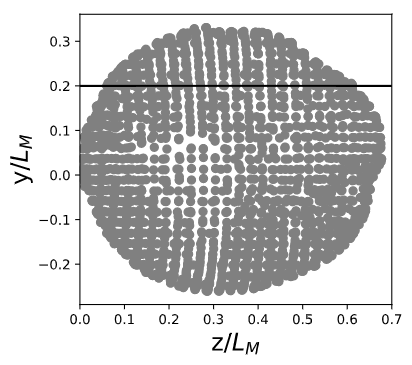
\includegraphics[width = 0.6\columnwidth]{./figure/Measure/SetLine.png}
	\caption{The border line to use a point cloud in the experiment.}
	\label{fig:Border}
\end{figure}  
\chcolor{The simulations aim to confirm that the propose method whether a two-piece brassiere cup can be designed to approximate an undevelopable surface that manifests the function of “fitting to a breast” .\rfig{fig:ObtainedSurfaceNDS2} shows the obtained shape and input data of experiments,  \rfig{fig:ObtainedSurfaceNDS2_Pat} shows the obtained pattern. In \rfig{fig:ObtainedSurfaceNDS2} and \rfig{fig:ObtainedSurfaceNDS2_Pat}, we set $ L_M = 72.8$. } \chcolor{\rtab{tbl:error and calc2} shows the error and calculation time of the experiment. From the result, we confirm that our proposed method also can design a two-piece brassiere cup to approximate data points under the conditions.
Hence, we conclude our proposed method in this paper is useful for the efficient design of paper patterns of a two-piece brassiere cup.}
\begin{table}[!h]
	\centering
	\begin{tabular}{|c|c|} \hline
		Error & Time[sec] \\ \hline
		1.04& 1682 \\ \hline
	\end{tabular}
	\caption{The error and calculation time of the proposed method in experiment.}
	\label{tbl:error and calc2}
\end{table}

\begin{figure}[h]
	\centering
	\subfigure[zx-view]{
		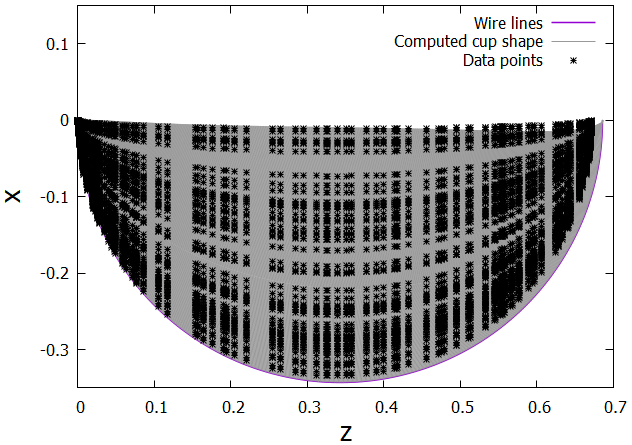
\includegraphics[width=0.6\columnwidth]{./figure/DS/ObtainedRidgeLinefromz-x.png}
		\label{fig:zx-DS}
	}
	\hfil
	\subfigure[zy-view]{
		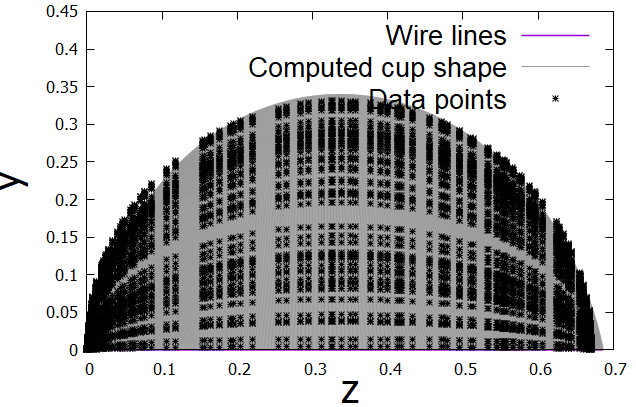
\includegraphics[width=0.6\columnwidth]{./figure/DS/ObtainedRidgeLinefromz-y.png}
		\label{fig:zy-DS}
	}
	\hfil
	\subfigure[zy-view]{
		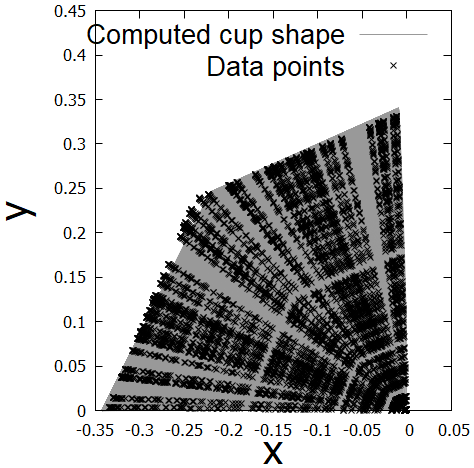
\includegraphics[width=0.6\columnwidth]{./figure/DS/ObtainedRidgeLinefromx-y.png}
		\label{fig:xy-DS}
	}
	\caption{Obtained shape and input data points in Case(2)}
	\label{fig:ObtainedSurfaceDS}
\end{figure}

\begin{figure}[h]
	\centering
	\subfigure[Lower pattern]{
		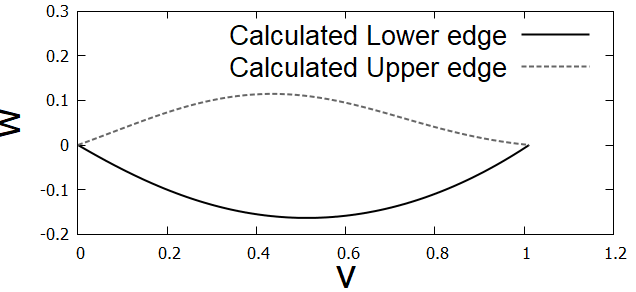
\includegraphics[width=0.6\columnwidth]{./figure/DS/ObtainedPatternL.png}
		\label{fig:low-DS}
	}
	\hfil
	\subfigure[Upper pattern]{
		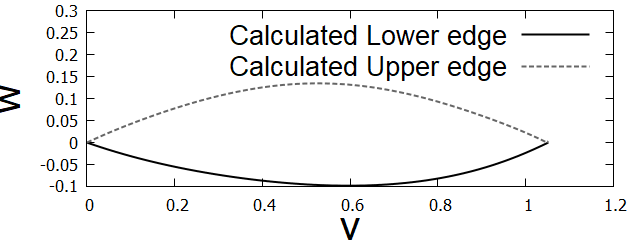
\includegraphics[width=0.6\columnwidth]{./figure/DS/ObtainedPatternU.png}
		\label{fig:upp-DS}
	}
	\caption{Obtained patterns in Case(1)}
	\label{fig:ObtainedSurfaceDS_Pat}
\end{figure}

\begin{figure}[h]
	\centering
	\subfigure[zx-view]{
		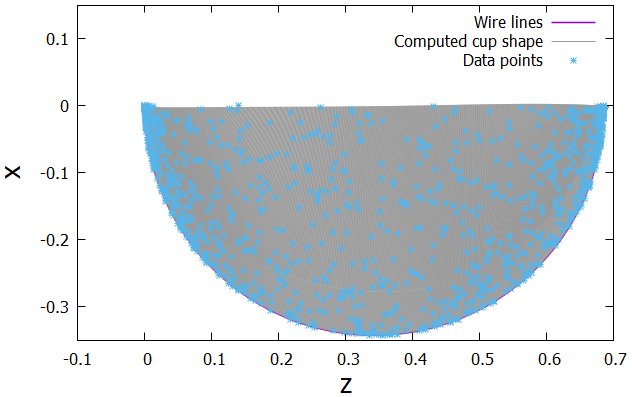
\includegraphics[width=0.6\columnwidth,clip]{./figure/NDS/ObtainedRidgeLinefromz-x.png}
		\label{fig:zx-NDS}
	}
	\hfil
	\subfigure[zy-view]{
		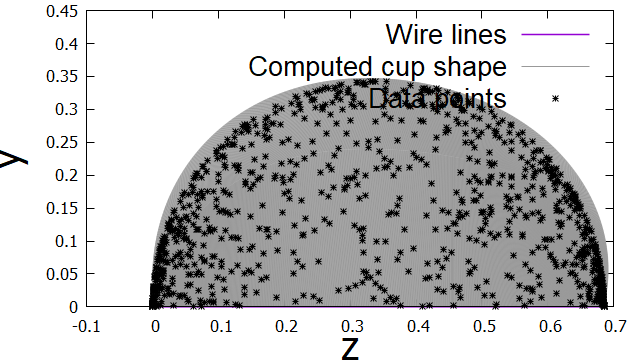
\includegraphics[width=0.6\columnwidth]{./figure/NDS/ObtainedRidgeLinefromz-y.png}
		\label{fig:zy-NDS}
	}
	\hfil
	\subfigure[xy-view]{
		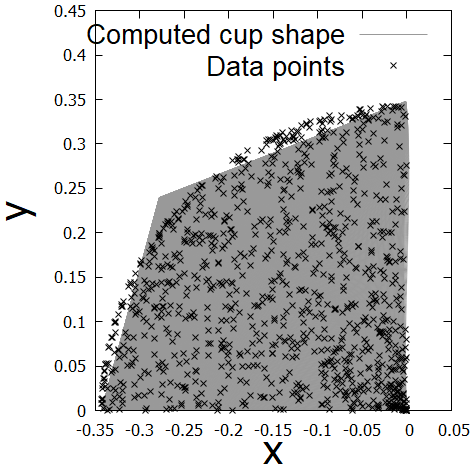
\includegraphics[width=0.6\columnwidth]{./figure/NDS/ObtainedRidgeLinefromx-y.png}
		\label{fig:xy-NDS}
	}
	\caption{Obtained shape and input data points in Case(2)}
	\label{fig:ObtainedSurfaceNDS}
\end{figure}

\begin{figure}[h]
	\centering
	\subfigure[Lower pattern]{
		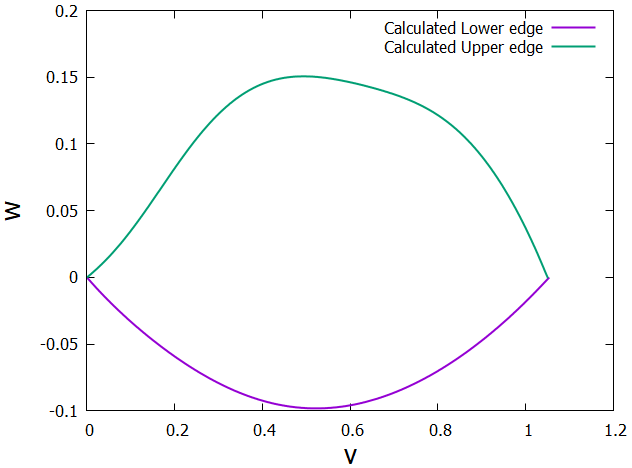
\includegraphics[width=0.6\columnwidth]{./figure/NDS/ObtainedPatternL.png}
		\label{fig:low-NDS}
	}
	\hfil
	\subfigure[Upper pattern]{
		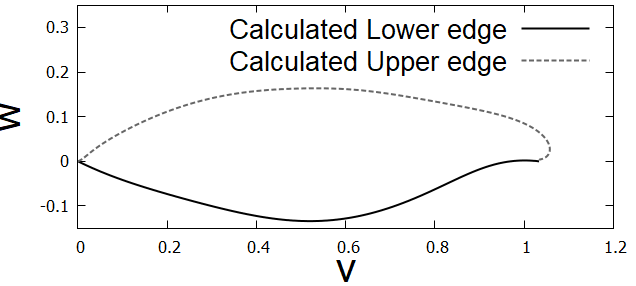
\includegraphics[width=0.6\columnwidth]{./figure/NDS/ObtainedPatternU.png}
		\label{fig:upp-NDS}
	}
	
	\caption{Obtained patterns in Case(2)}
	\label{fig:ObtainedSurfaceNDS_Pat}
\end{figure}

\begin{figure}[H]
	\centering
	\subfigure[zx-view]{
		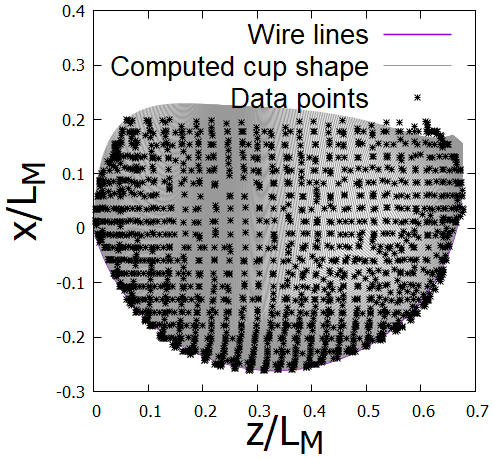
\includegraphics[width=0.6\columnwidth]{./figure/Measure/ObtainedRidgeLinefromz-x.png}
		\label{fig:zx-NDS2}
	}
	\hfil
	\subfigure[zy-view]{
		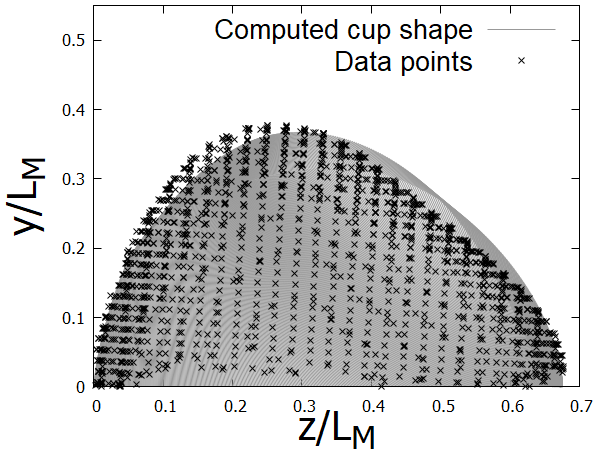
\includegraphics[width=0.6\columnwidth]{./figure/Measure/ObtainedRidgeLinefromz-y.png}
		\label{fig:zy-NDS2}
	}
	\hfil
	\subfigure[xy-view]{
		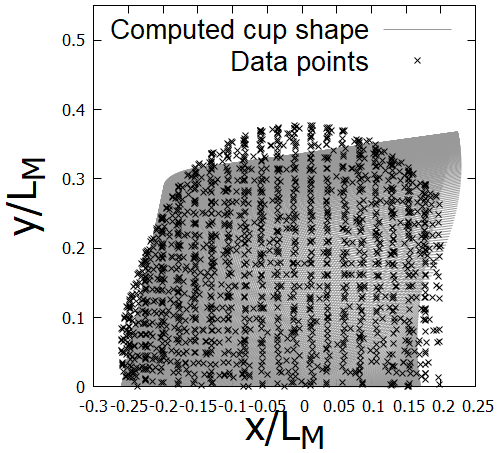
\includegraphics[width=0.6\columnwidth]{./figure/Measure/ObtainedRidgeLinefromx-y.png}
		\label{fig:xy-NDS2}
	}
	\caption{Obtained shape and input data points in the experiment}
	\label{fig:ObtainedSurfaceNDS2}
\end{figure}

\begin{figure}[h]
	\centering
	\subfigure[Lower pattern]{
		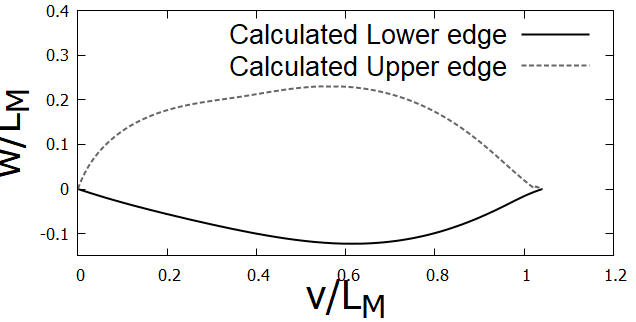
\includegraphics[width=0.6\columnwidth]{./figure/Measure/ObtainedPatternL.png}
		\label{fig:low-NDS2}
	}
	\hfil
	\subfigure[Upper pattern]{
		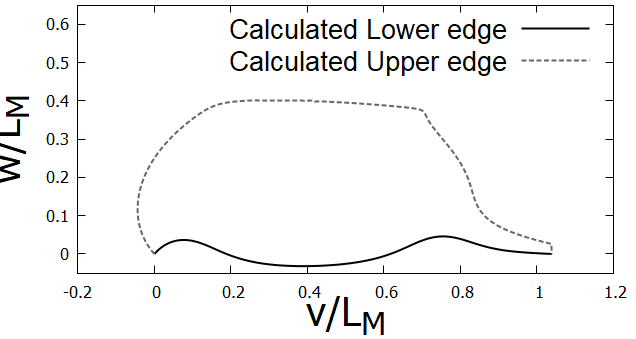
\includegraphics[width=0.6\columnwidth]{./figure/Measure/ObtainedPatternU.png}
		\label{fig:upp-NDS2}
	}
	
	\caption{Obtained patterns in the experiment}
	\label{fig:ObtainedSurfaceNDS2_Pat}
\end{figure}


\section*{CONCLUSION}
\subsection*{Summary}
Herein we propose a method to design the shape of a two-piece brassiere cup and its patterns to satisfy the function of "fitting to a breast shape" when the shape is given as a cloud of data points. In the typical design process, a cup model is made of paper to verify the pattern shape. Our model assumes that the model surface is comprised of several developable surfaces. First, we formulate the cup model based on differential geometry and hypothesize that a developable surface can be determined by two curves included in it. Hence, the design process of a two-piece brassiere cup can be converted into an optimization problem, whose objective function is the error between the cup shape and its data points. To calculate the error, first the error between a point and the surface from the geometry condition is formulated. Second, our proposed method divides the data cloud into two: the lower and upper cups. Then the cups are evaluated. To verify our proposed method, we assessed two cases. One is a non-developable surface, and the other is a developable surface. The results confirm that the proposed method can design a cup shape, which manifests the intended function. Consequently, our proposed method should be useful to efficiently design a two-piece brassiere cup. 
\subsection*{Limitation and Future Work}
\chcolor{Though we proposed a method to design the shape of a two-piece brassiere cup and its patterns to satisfy the function of "fitting to a breast shape" when the shape is given as a cloud of data points, there is still a  question from the point of view of real-world applications. This is whether the brassire cup should cover the breast shape. A brassire cup has several demands, which include the function to form the ideal breast shape. So the function of "fitting to a breast shape" does not only mean fitting to a breast shape itself, but also fitting to an ideal breast shape one wants. For future work, to quantify how much fitting a breast shape and controll it are required.}
%a this paper, a method to design the cup shape of two-piece brassiere cup and its patterns was proposed when its target shape is given as a cloud of data points. As a cup model for check of the shapes of patterns is made of paper, it is assumed that the surface of the model is composed of several developable surfaces. We claimed that a developable surface can be determined by two curves included in it. The design process of a two-piece brassiere cup can be converted to the optimization problem, whose objective function is the error between the cup shape and its data points. In order to calculate the error, we proposed a method to divide a data cloud into two clouds: evaluated by the lower cup, or evaluated by the upper cup. It was experimentally verified that the cup shape calculated by our proposed method reproduced the given data points well. Our proposed method will be useful for efficient design of not only patterns of a brassiere cup but also plate parts of a structure consisting of developable surfaces.

%%%%%%%%%%%%%%%%%%%%%%%%%%%%%%%%%%%%%%%%%%%%%%%%%%%%%%%%%%%%%%%%%%%%%%
%\bibliography{asme2ebackup}

\begin{thebibliography}{99}
	
	\bibitem{c1}Yukiko Higuchi, {\it Sensory test of brassiere}, in The Japanese Journal of Ergonomics, Volume 20, Issue 2, 1984, pp.73-80, (Japanese).
	\bibitem{c2} P.Bo and W.Wang, {\it "Geodesic-Controlled Developable Surfaces for Modeling Paper Bending"}, in Computer Graphics Forum, Volume 26, 2007, pp.365-374.
	\bibitem{c3} H.Pottmann and J.Wallner, {\it "Approximation algorithms for developable surfaces"}, in Computer Aided Geometric Design, Volume 16, 1999, pp.539-556.
	\bibitem{c4} K.Rose, A.Sheffer, J.Wither, M.Cani, and B.Thibert, {\it "Developable surfaces from arbitrary sketched boundaries"}, SGP ’07 Proceedings of the fifth Eurographics symposium on Geometry processing, 2007, pp.163-172.
	\bibitem{c5} G.Aumann, {\it "A simple algorithm for designing developable Bezier surfaces"}, in Computer Aided Geometrix Design Volume 20, 2003, pp.601-619.
	\bibitem{c6} B.Ravani and T.S. Ku, {\it "Bertrand offsets of ruled and developable surfaces"} in Computer-Aided Design Volume 23, 1991, pp.145-152. 
	\bibitem{c7}R.M.C Bodduluri and B.Ravani, {\it "Design of developable surfaces using duality between plane and point geometries"}, in Computer Aided Design Volume 25, 1993, pp.621-632.
	\bibitem{c8}M. Peternell, {\it "Developable surface fitting to point clouds"}, in Computer Aided Design Vol.21, 2004, pp.785-803.
	\bibitem{c9}H.-Y. Chen, I.-K. Lee, S. Leopoldseder, H. Pottmann, T. Randrup , J. Wallner, {\it "On Surface Approximation using Developable Surfaces"}, Graphical Models and Image Processing, Volume 61, Issue2, 1999, pp.110-124
	\bibitem{cX1} Y. Liu, H. Pottmann, J. Wallner, Y.-L. Yang, and W. Wang, {\it "Geometric modeling with conical meshes and developable surfaces"}, Proc.Int. Symp. SIGGRAPH, 2006, pp.681-689
	\bibitem{cX2} O. Stein, E. Grinspun, and K. Crane, {\it Developability of triangle meshes}, ACM Transaction on Graphics, Vol.37, Issue4, 2018, pp77:1-14
	\bibitem{cX3} M. Kilian, S. Flöry, Z. Chen, N. J. Mitra, A. Sheffer, and H. Pottmann, {\it Curved folding}, ACM Transaction on Graphics, Vol.27, Issue3, 2008, pp1-9
	\bibitem{c10} H.Wakamatsu, Y.Ryu, E.Morinaga, E.Arai, and T. Kubo, M.Oyama, and T.Kishimoto, {\it "3D Shape Prediction of A Paper Model of Two Piece Brassiere Cup for Its Efficient Design"}, Proc.Int. Symp. Flexible Automation, 2016, pp.326-332
	\bibitem{c11} H.Wakamatsu, E.Morinaga, E.Arai, and T. Kubo, {\it "A Virtual Paper Model of a Three Piece Brassiere Cup to Improve the Efficiency of Cup Design Process"}, Proc. 2017 IEEE Int. Conf. on Robotics and Automation, 2017. 
	\bibitem{c12}M.Itoh, and H.Imaoka, {\it "A Method of Prediction Sewn Shapes and a Possibility of Sewing by the Theory of Developable Surfaces"}, J. the Japan Research Association for Textile End-Uses, Volume 48, 2007, pp.42-51, (Japanese).
	\bibitem{MyRef} Kotaro Yoshida, Hidefumi Wakamatsu, Eiji Morinaga, Eiji Arai, Seiichiro Tsutsumi, Takahiro Kubo,{\it "Pattern Shape Optimization of a Two-piece brassiere cup to improve its design efficiency"}, Trans. of the Institute of Systems, Control and Information Engineers, Volume 32, No. 5, 2019, pp. 192-202.
	\bibitem{MyRef2} Kotaro Yoshida, Hidefumi Wakamatsu, Eiji Morinaga, Seiichiro Tsutsumi, and Takahiro Kubo, {\it Design support of a developable surface considering its bending energy}, Transaction of the JSME, Vol.86, No.890, 2020, pp20-36(in Japanese)
	\bibitem{cX4} S. Kobayashi, {\it "Differential Geometry of Curves and Surface"}, Shokado, Tokyo, 1995, Chap2 (in Japanse)
	\bibitem{c13}Elsgolc L.E {\it Calculus of Variations}, Pergamon Press, 1961, pp. 144-157.
\end{thebibliography}

\authorbiography{Kotaro, YOSHIDA}{}{Non-Member}{%
	Kotaro Yoshida received his B.Eng. and M.Eng. degree from Osaka University in 2017 and 2019, respectively. He is doing a doctoral degree at Osaka University.
}

\authorbiography{Hidefumi, ,WAKAMATSU}{}{Member}{%
	HidefumiWakamatsu received his B.Eng.,
	M.Eng. and Ph.D. degrees from Osaka
	University, Japan, in 1993, 1994 and
	2001, respectively. From 1995 to 2006,
	he worked as a Research Associate, Osaka
	University. He then became an Associate
	Professor at Division of Materials and Manufacturing
	Science, Osaka University. His research interests
	include handling of flexible object. He is a member of
	RSJ, JSME, JSPE, JWS and TMSJ.
}

\authorbiography{Eiji, ,MORINAGA}{}{Member}{%
	Eiji Morinaga received his B.Eng., M.Eng.
	and Ph.D. degrees in Mechanical Engineering
	from Osaka University, Japan,
	in 2000, 2002 and 2005, respectively. From
	2005 to 2007, he worked as a Designated
	Researcher at Center for Advanced Science
	and Innovation, Osaka University. He then became
	an Assistant Professor at Division of Materials and Manufacturing
	Science, Osaka University. His research interests
	include system design and integration in product design
	and manufacturing. He is a member of JSME, JSPE,
	JWS, JIEP and TMSJ.
}

\authorbiography{Takahiro, ,KUBO}{}{Non-Member}{%
	Takahiro Kubo received his B.A. degree in Sport Sciences from Waseda University, Japan, in 2007, and M.A. degree in Arts and Sciences from Tokyo University, Japan, in 2010. He then joined Wacoal Corp. His position is in Human Science Research Center.
}


\end{document}
%
%% end of paper.tex
